148. \begin{figure}[ht!]
\center{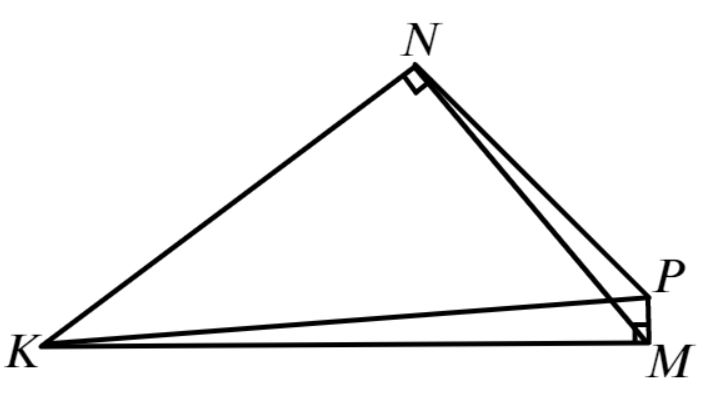
\includegraphics[scale=0.35]{g9-148.png}}
\end{figure}\\
Найдём $\angle K=360^\circ-90^\circ-90^\circ-120^\circ=60^\circ.$ Тогда по теореме косинусов $NM^2=16+36-2\cdot4\cdot6\cdot\cfrac{1}{2}=28,\ BD=2\sqrt{7}$ и $16=36+28-2\cdot6\cdot2\sqrt{7}\cos(\angle KNM),\ \cos(\angle KNM)=\cfrac{2}{\sqrt{7}}.$ Так как $\angle N+\angle N=180^\circ,$ четырёхугольник $MKNP$ является вписанным и $\angle KPM=\angle KNM.$ Найдём $\sin(\angle KPM)=\sqrt{1-\cfrac{4}{7}}=\cfrac{\sqrt{3}}{\sqrt{7}}=\cfrac{KM}{PK}=\cfrac{4}{PK},$ откуда $PK=\cfrac{4}{3}\sqrt{21}.$\\
